%!TEX root = ../main.tex
\setcounter{chapter}{-1}
\chapter{Introduction and system model.}
%
\section{Introduction}
	With the case study of the course \emph{Multivariable Control and Coordination Systems}, we aim at putting into practice the concepts and methodologies presented in the lectures, as well as at providing a quick glance at how Matlab-Simulink can be used to simulate dynamical systems and implement and assess control strategies. \par
	%
	Four exercises are proposed, all of them somewhat related to some of the control challenges connected to self-driving cars technology.
	Specifically, we will address the problems of path tracking and trajectory and path planning problems. 
	Path tracking consists in controlling the vehicle so that it accurately tracks a predefined path of interest. 
	Trajectory planning deals with the task of planning, in a certain temporary horizon, a sequence of control actions that will make the vehicle avoid collision and track the desired path. 
	Similarly, path planning deals with the calculation of the path to be followed without considering any temporary information.
	The mentioned problems are complex in reality and we will tackle here simplified versions of them. \par
	%
	We will begin by implementing and assessing the linear-model-based control and observation techniques described in the course.
	Namely we will discuss regarding the usefulness and limitations of linear-model-based control techniques, LQR control design and implementation, and observers.
	Then, we will make use of the dynamic programming concept and the Bellman's principle of optimality to address the trajectory planning problem through a graph-search algorithm.
	Finally, path planning will be tackled with a navigation function-based technique.
	%
	\paragraph{Files}
	In every exercise session you will be provided with the description of the exercise, a Matlab script \texttt{exercise\#\_*.m} (which does not need to be modified), a Matlab class \texttt{utilities.m} (common to all exercises) gathering some auxiliary functions the exercise scripts will use, a Matlab-class named \texttt{ex\#.m} which will include the functions that you have to complete, as well as simulink files which also have to be completed.\par
	%
	The fact that we are using a class to gather the functions you have to complete is simply for clarity proposes. 
	The methods of such a class will then be called from the provided exercise script.\par
	%
	%Basic Matlab 
	%Although not too advanced Matlab skills are needed to complete the exercises, they will definitely come in handy to understand the provided code, and how the functions are integrated in the main script.\par
	%
	\paragraph{Evaluation}
	At the end of the course we expect you to submit a zip file (named \texttt{Surname-Name.zip}) with a total of 8 items:
	\begin{itemize}
		\setlength\itemsep{0em}
		%
		\item A pdf document reporting the results and discussions of all the proposed exercises. 
		\item Four \texttt{ex\#.m} files, one per session, containing your solutions to the proposed exercises. 
		\item Three Simulink files with the block diagrams used to run the experiments.
	\end{itemize}
	Even though we encourage you to work in small groups (preferably up to 3 people) and to discuss ideas to overcome the difficulties you might find, the report \textbf{must} be written individually. 
	Please keep in mind that assessing simulation results is crucial and a bad/good discussion can invalidate/validate good/bad results. 	
	%
	Important: although the matlab and simulink files are requested, \textbf{the evaluation of the exercises will be solely based on the pdf report}.
	Meaning that references in the pdf document such as "as can be seen in the attached simulink file" or others of the sort must be avoided. 
	Do not expect us exploring the Matlab files to find the solutions.
	Everything you want us to take into account when grading the exercises must be included in the report. 
	The only propose of requesting the Matlab files is guaranteeing the uniqueness of your solution.\par
	%
	Please notice that this is the first iteration of this case study as it is presented this year. 
	Therefore, it exists the probability of finding bugs, typos, or inconsistencies in the code. 	
	We kindly ask you to point out any flaw you find so that we can improve and update the material of the case study over the year, converging to a more robust version of it.
	%
\section{The model}
	%
	To tackle the control/planning problems here-above mentioned, we are going to make use of the so-called kinematic bicycle model of a car, described by the next set of differential equations
	\begin{subequations}
	\begin{align}
		\dxPos 		& = \speed\cos(\yaw) \\
		\dyPos 		& = \speed\sin(\yaw) \\
		\dyaw 		& = \frac{\speed}{\carLength}\tan(\steering) \\
		\dspeed     & = \accDyn(\alpha-\speed)\\
		\dsteering & = \steerDyn(\beta-\steering)
		%\dot{\steeringRef} & = \alpha\\
		%  & = \\
	\end{align}
	\end{subequations}
	where $\xPos, \xPos, \yaw$ represent the absolute position and orientation of the vehicle w.r.t a fixed frame of reference, $\speed$ denotes the \emph{longitudinal} speed, $\carLength$ denotes the car length,  $\steering$ shows the steering wheel angle, $\alpha$ and $\beta$ show the speed and the steering wheel angle reference (control inputs), and $\accDyn$ and $\steerDyn$ represent the dynamic of the actuators in charge of tracking longitudinal speed and steering wheel angle references.\par
	%
	A common practice to perform path tracking consists in rewriting the system in such a way that the position is expressed w.r.t. the path that should be followed (as it is illustrated in Fig \ref{fig:system}).
	Technique which reveals itself very useful when constant-curvature paths (or paths resulting from the concatenation of constant-curvature segments) are followed.
	The technique consists in expressing the position of the vehicle through the curvilinear coordinate $\pathCoor$, the \emph{lateral deviation w.r.t. the path of reference} $\distToPath$, as well as the \emph{heading error} $\yawErr$ (see Fig. \ref{fig:system} for a better understanding of the introduced states).\par
	%
	\begin{figure}[!h]
		\centering
		\resizebox{ 300 px }{!}{
			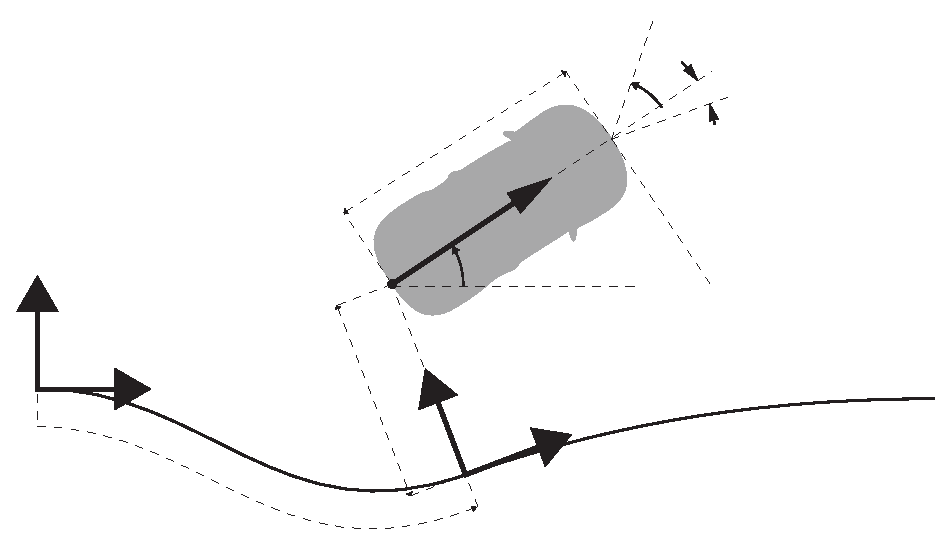
\includegraphics[width = 250px]{./_imags/system}
			\put(-187,0){$\pathCoor$}
			\put(-163,30){$\distToPath$}
			\put(-55,110){$\yawErr$}
			\put(-77,121){$\steering$}
			\put(-127,70){$\yaw$}
			\put(-132,85){$\speed$}
			\put(-142,105){$\carLength$}
		}
		\caption{Coordinate and variable representation of the path tracking problem}
		\label{fig:system}
	\end{figure}	
	%
	The car model can then be reformulated as follows:
	\begin{subequations}
	\begin{align}	
		%\dxPos 		& = \speed\cos(\yaw) \\
		%\dyPos 		& = \speed\sin(\yaw) \\
		%\dyaw 		& = \frac{\speed}{\carLength}\tan(\steering) \\	
		\dpathCoor 	& = \frac{\speed\cos(\yawErr)}{1-\distToPath\curvature} \label{eq:non_linear_model_1}\\
		\ddistToPath& = \speed\sin(\yawErr) \label{eq:non_linear_model_2}\\
		\dyawErr    & = \frac{\speed}{\carLength}\tan(\steering) - \curvature\dpathCoor \label{eq:non_linear_model_3}\\
		\dspeed & = \accDyn(\alpha-\speed) \label{eq:non_linear_model_4}\\
		\dsteering & = \steerDyn(\beta-\steering) \label{eq:non_linear_model_5}
	\end{align}
	\end{subequations}
	where $\curvature$ shows the path curvature w.r.t. the path coordinate $\pathCoor$.
	Looking at equations \ref{eq:non_linear_model_1}-\ref{eq:non_linear_model_5} it becomes evident why constant-curvature paths are desired. 
	Mainly because of the fact that the tracking problem becomes much more easy to handle.
	For the sake of simplicity, we are going to assume that the path has a constant curvature. %\par
	%
	Moreover, we will consider the state-space vector, and control inputs to be 
	\begin{align}
		\mathbf{\state} & = \left[ \stat{1},\stat{2},\stat{3},\stat{4},\stat{5}\right] = %
							\left[\pathCoor, \distToPath, \yawErr, \speed, \steering\right] \label{eq:stateVector}\\ 
		\mathbf{\control} & = \left[ \con{1},\con{2} \right] = %
							  \left[ \alpha, \beta \right].
	\end{align}
	which would then allow us to rewrite the model in the form $ \mathbf{\dot{\state}} = f(\mathbf{\state},\mathbf{\control},t) $ as
	\begin{align}
		%
		%\dstat{1} 	& = \stat{7}\cos(\stat{3})\\
		%\dstat{2} 	& = \stat{7}\sin(\stat{3})\\
		%\dstat{3} 	& = \frac{\stat{7}}{L}\tan{\stat{8}}\\
		%
		\dstat{1} 	& = \frac{\stat{4}\cos(\stat{3})}{1-\stat{2}\curv} \label{eq:ss1}\\
		\dstat{2}   & = \stat{4}\sin(\stat{3}) \label{eq:ss2}\\
		\dstat{3}   & = \frac{\stat{4}}{\carLength}\tan(\stat{5}) - \frac{\curv\stat{4}\cos(\stat{3})}{1-\stat{2}\curv} \label{eq:ss3}\\
		\dstat{4}   & = \accDyn(\con{1}-\stat{4})\label{eq:ss4}\\
		\dstat{5}   & = \steerDyn(\con{2}-\stat{5}) \label{eq:ss5}
	\end{align}
	%
	which is the continuous non-linear model of the system we will use to implement linear-model-based control and observation techniques in the following exercises. 
		



